\documentclass{article}
\usepackage[utf8]{inputenc}
\usepackage[T1]{fontenc}
\usepackage[french]{babel} 
\usepackage{graphicx}

\title{Lab 1 - Global States and Distributed Snapshots}

\author{
  Ruben Mbiyavanga \and
  Nassir Naibi \and
  Louis Poutrain \and
  Gregory Dubouloy
}


\date{\today}

\begin{document}

\maketitle 

\tableofcontents 

\newpage

\section{Introduction}

Ce rapport présente l'implémentation d'un simulateur d'exécution distribuée basé sur l'algorithme \textit{Chandy-Lamport} pour capturer des snapshots globaux cohérents. Le projet inclut deux interfaces utilisateur (formulaire et graphique) permettant de concevoir et d'exécuter des simulations, ainsi qu'une visualisation espace-temps pour l'analyse.

\section{Architecture et Implémentation}

\subsection{Composants}

Le projet s'organise autour de quatre modules : \textbf{Simulator} (orchestration, file d'événements), \textbf{Process} (état local, implémentation Chandy-Lamport), \textbf{Message} (type APP/MARKER), \textbf{Event} (tuple $(timestamp, action)$).

\subsection{Algorithme}

\begin{enumerate}
    \item L'initiateur enregistre son état et marque tous les canaux entrants.
    \item Des marqueurs sont envoyés à tous les voisins.
    \item À réception du premier marqueur : enregistrement de l'état et des autres canaux.
    \item Messages reçus avant le marqueur sont capturés dans l'état du canal.
\end{enumerate}

\newpage

\section{Exemple Consistant}

\subsection{Description}

Notre exemple met en avant une exécution distribuée avec la propriété suivante : dans la coupure réalisée, \textbf{toute conséquence détectable a une causalité causale capturable}.

\subsection{Scénario}

Considérons 3 processus $P_1$, $P_2$, $P_3$ avec la topologie mesh (tous connectés). Le scénario suit ces étapes :

\begin{enumerate}
    \item $t=1$ : $P_3$ envoie un message à $P_2$ (Msg 3→2).
    \item $t=2$ : $P_1$ envoie un message à $P_2$ (Msg 1→2).
    \item $t=6$ : $P_1$ initie le snapshot global.
    \item $t=8$ : $P_2$ envoie un message à $P_1$ (Msg 2→1, message critique).
    \item $t=15$ : $P_1$ envoie un message à $P_4$ (Msg 1→4).
    \item $t=20$ : $P_1$ envoie un message à $P_3$ (Msg 1→3).
\end{enumerate}

Le message critique $P_2 \to P_1$ au temps $t=8$ est reçu après le démarrage du snapshot en $P_1$ (t=6) et avant la réception du marqueur de retour. Ce message est donc correctement capturé par le snapshot.

La coupure est consistante car tout message ayant une conséquence observable est enregistré en tant que message en transit.

\begin{figure}[h]
    \centering
    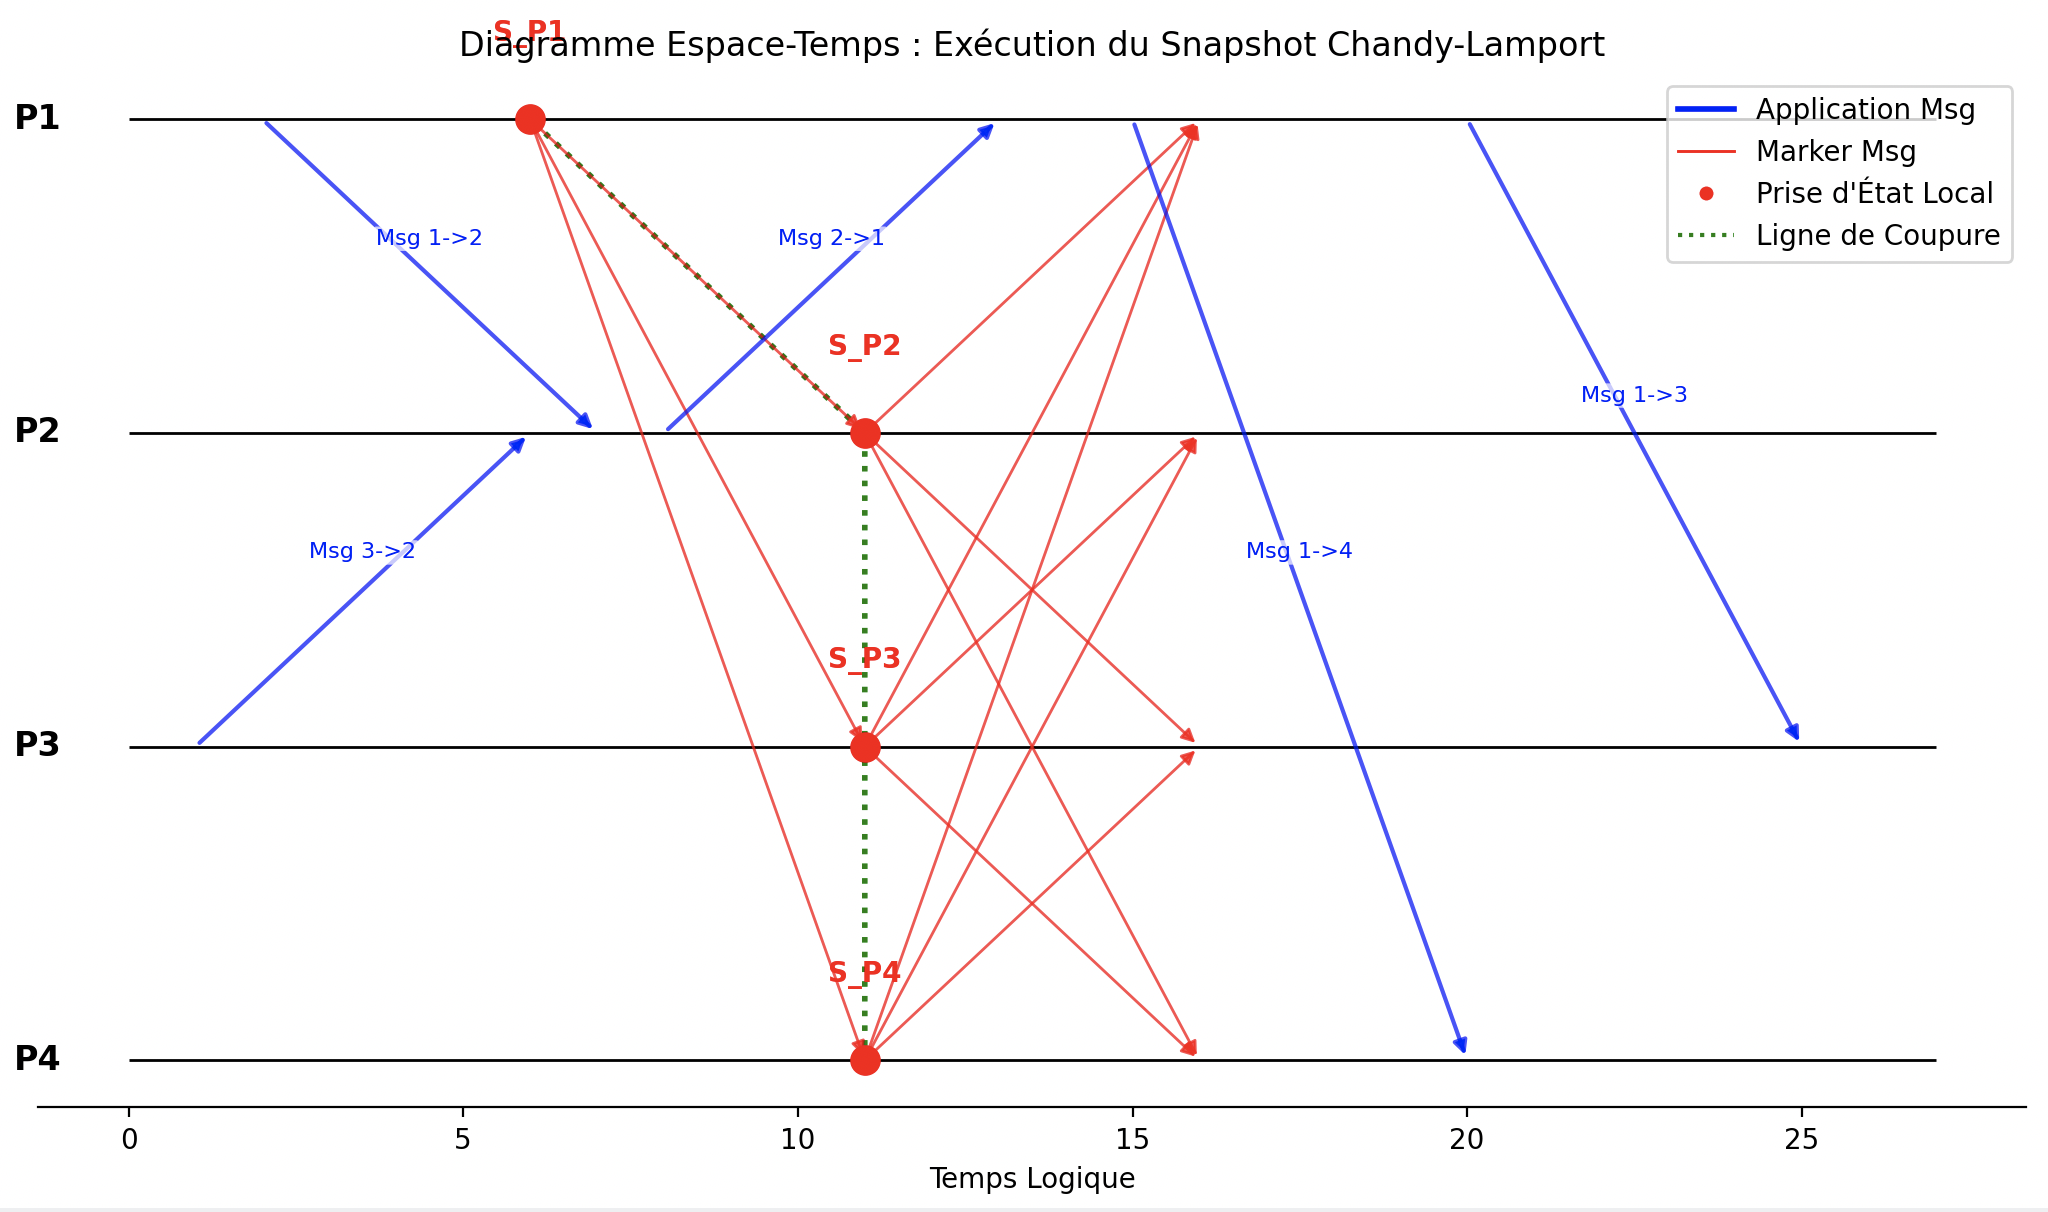
\includegraphics[width=0.85\linewidth]{Images/Capture_decran_2026-01-27_a_15.45.00.png}
    \caption{Diagramme espace-temps : snapshot Chandy-Lamport avec message critique.}
    \label{fig:execution}
\end{figure}

\newpage

\section{Interfaces et Résultats}

\subsection{Interface Formulaire (ui.py)}

Champs texte pour processus, tableaux pour ajouter/supprimer messages et snapshots. Idéale pour tests rapides.

\subsection{Interface Graphique (ui\_graphical.py)}

Diagramme espace-temps interactif : insertion de messages (clic source → clic destination), snapshots (clic processus), visualisation immédiate.

\subsection{État Global Capturé}

Pour chaque processus, on enregistre :
\begin{itemize}
    \item Son état local au moment du snapshot.
    \item L'état de chaque canal entrant (messages en transit).
\end{itemize}

\subsection{Exemple de Résultat}

\begin{verbatim}
Processus P1:
  État Local: 3
  Canaux entrants :
    From P2: ['Msg 2->1']
    From P3: <Vide>

Processus P2:
  État Local: 5
  Canaux entrants :
    From P1: <Vide>
    From P3: ['Msg 3->2']
\end{verbatim}

Ce résultat valide la consistance de la coupure : le message critique de $P_2$ vers $P_1$ est bien capturé.

\section{Conclusion}

Ce projet implémente avec succès l'algorithme \textit{Chandy-Lamport} pour capturer des snapshots globaux cohérents. Les deux interfaces (formulaire et graphique) offrent une grande flexibilité d'utilisation. L'approche garantit la consistance des coupures dans un système asynchrone sans horloge globale.

\end{document}